%%%%%%%%%%%%%%%%%%%%%%%%%%%%%%%%%%%%%%%%%%%%%%%%%%%%%%%%%%
%
% Vzor pro sazbu kvalifikační práce
%
% Západočeská univerzita v Plzni
% Fakulta aplikovaných věd
% Katedra informatiky a výpočetní techniky
%
% Petr Lobaz, lobaz@kiv.zcu.cz, 2016/03/14
%
%%%%%%%%%%%%%%%%%%%%%%%%%%%%%%%%%%%%%%%%%%%%%%%%%%%%%%%%%%

% Možné jazyky práce: czech, english
% Možné typy práce: BP (bakalářská), DP (diplomová)
\documentclass[czech,BP]{thesiskiv}

% Definujte údaje pro vstupní strany
%
% Jméno a příjmení; kvůli textu prohlášení určete, 
% zda jde o mužské, nebo ženské jméno.
\author{Hinterholzinger Jan}
\declarationmale

%alternativa: 
%\declarationfemale

% Název práce
\title{Softwarová podpora organizace předmětů TSP}

% 
% Texty abstraktů (anglicky, česky)
%
\abstracttexten{The text of the abstract (in English). It contains the English translation of the thesis title and a short description of the thesis.}

\abstracttextcz{Text abstraktu (česky). Obsahuje krátkou anotaci (cca 10 řádek) v češtině. Budete ji potřebovat i při vyplňování údajů o bakalářské práci ve STAGu. Český i anglický abstrakt by měly být na stejné stránce a měly by si obsahem co možná nejvíce odpovídat (samozřejmě není možný doslovný překlad!).
}

% Na titulní stranu a do textu prohlášení se automaticky vkládá 
% aktuální rok, resp. datum. Můžete je změnit:
%\titlepageyear{2016}
%\declarationdate{1. března 2016}

% Ve zvláštních případech je možné ovlivnit i ostatní texty:
%
%\university{Západočeská univerzita v Plzni}
%\faculty{Fakulta aplikovaných věd}
%\department{Katedra informatiky a výpočetní techniky}
%\subject{Bakalářská práce}
%\titlepagetown{Plzeň}
%\declarationtown{Plzni}

%%%%%%%%%%%%%%%%%%%%%%%%%%%%%%%%%%%%%%%%%%%%%%%%%%%%%%%%%%
%
% DODATEČNÉ BALÍČKY PRO SAZBU
% Jejich užívání či neužívání záleží na libovůli autora 
% práce
%
%%%%%%%%%%%%%%%%%%%%%%%%%%%%%%%%%%%%%%%%%%%%%%%%%%%%%%%%%%

% Zařadit literaturu do obsahu
\usepackage[nottoc,notlot,notlof]{tocbibind}

% Umožňuje vkládání obrázků
\usepackage[pdftex]{graphicx}

% Odkazy v PDF jsou aktivní; navíc se automaticky vkládá
% balíček 'url', který umožňuje např. dělení slov
% uvnitř URL
\usepackage[pdftex]{hyperref}
\hypersetup{colorlinks=true,
  unicode=true,
  linkcolor=black,
  citecolor=black,
  urlcolor=black,
  bookmarksopen=true}

% Při používání citačního stylu csplainnatkiv
% (odvozen z csplainnat, http://repo.or.cz/w/csplainnat.git)
% lze snadno modifikovat vzhled citací v textu
\usepackage[numbers,sort&compress]{natbib}

\usepackage{float}

% Barvičky
\usepackage{xcolor}
\colorlet{mygray}{black!30}
\colorlet{mygreen}{green!60!blue}
\colorlet{mymauve}{red!60!blue}
% Vkládání formátovaného zdrojového kódu
\usepackage{listings}
\renewcommand{\lstlistingname}{Ukázka kódu}
\renewcommand\lstlistlistingname{Seznam ukázek kódu}
\lstset{
	backgroundcolor=\color{gray!10},  
	basicstyle=\ttfamily,
	columns=fullflexible,
	breakatwhitespace=false,      
	breaklines=true,                
	captionpos=b,                    
	commentstyle=\color{mygreen}, 
	extendedchars=true,              
	frame=single,                   
	keepspaces=true,             
	keywordstyle=\color{blue},      
	language=php,                 
	numbers=none,                
	numbersep=5pt,
	numberbychapter=false,
	numberstyle=\tiny\color{blue}, 
	rulecolor=\color{mygray},        
	showspaces=false,               
	showtabs=false,
	showstringspaces=false,
	stepnumber=1,                  
	stringstyle=\color{mymauve},    
	tabsize=3,                      
	title=\lstname,
	numbers=left       
}

%%%%%%%%%%%%%%%%%%%%%%%%%%%%%%%%%%%%%%%%%%%%%%%%%%%%%%%%%%
%
% VLASTNÍ TEXT PRÁCE
%
%%%%%%%%%%%%%%%%%%%%%%%%%%%%%%%%%%%%%%%%%%%%%%%%%%%%%%%%%%
\begin{document}
%
\maketitle
\tableofcontents

V souboru \texttt{literatura.bib} jsou uvedeny příklady, jak citovat knihu \cite{KnuthAOCP2}, článek v časopisu \cite{Hoare1961}, webovou stránku \cite{Graphics2D}.
\chapter{Úvod}
\chapter{}
\section{Motivace}
	\par Na Katedře informatiky a výpočetní techniky vzniká nový předmět Týmový softwarový projekt (KIV/TSP1 a KIV/TSP2) určený pro studenty navazujícího studia. Podstatou předmětu je vypracování zadaného tématu ve skupinkách studentů, kdy studenti přijdou do styku s týmovou prací, řízením projektu a dalšími interními procesy.
	\par Zvláštností předmětu je doba pro řešení projektu, dva semestry rozdělené do dvou předmětů. Budou zapojeny čtyři skupiny lidí. Garant, zadavatelé, mentoři a studenti, což bude klást poměrně značné nároky na organizaci předmětu. Pro takový rozsah bylo rozhodnuto o vytvoření webové aplikace, která všem zúčastněným stranám zjednoduší prohlížení obsahu a evidenci postupu prací projektu. Cílem aplikace je umožnit lepší informovanost a zapojení studentů, řešení evidence zadavatelů a možnosti sdílení mezi mentorem a garantem. Aplikace tak má nahradit způsob organizace pomocí Excel tabulky, jako je tak tomu u jiných obdobných předmětů.
\chapter{Specifikace požadavků}
\section{Organizace předmětů TSP}
	\par Výuka předmětů TSP je rozdělena do dvou semestrů, a tedy do dvou předmětů KIV/TSP1 vyučovaného v letním semestru 1. ročníku a KIV/TSP2 v zimním semestru 2. ročníku. Řešení týmového projektu tedy bude překračovat hranice ročníku a v mnoha částech se organizace předmětů bude překrývat.
	\par Jednotlivý cyklus se v nejčastějším případě bude probíhat následovně. 
	\begin{itemize}
		\item Garant přijímá od domluvených zadavatelů jejich témata, která mají studentské týmy řešit. Toto zadání společně s možným PDF souborem vloží do podpůrného softwaru pro zvolené období předmětu.
		\item Před začátkem TSP budoucí vedoucí týmu zažádá garanta o založení účtu v podpůrném softwaru s rolí \uv{Vedoucí}. Vedoucí týmu společně s dalšími studenty sestaví tým a vloží informace o týmu do této podpory.
		\item Poté co jsou témata zadání projektů zveřejněny, vedoucí týmu (na základě rozhodnutí v týmu) projeví zájem o zvolené téma.
		\item Mentor ohodnotí vhodnost zvoleného tématu pro daný tým na základě zájmu, který vedoucí týmu učinil.
		\item Garant následně podle rozhodnutí mentora a zájmu týmu definitivně přiřadí nebo nepřiřadí téma týmu. Přiřazením tématu vzniká projekt.
		\item Tým řeší projekt a postup řešení vkládá do softwarové podpory
		\item Mentor na základě postupu řešení týmu kontroluje a potvrzuje postup týmu
		\item Na závěru předmětu TSP se koná obhajoba projektu, jejíž výsledek se zapíše do softwarové podpory.
	\end{itemize}
\section{Uživatelé}
	\subsection{Nepřihlášený uživatel}
		\par Nepřihlášený uživatel je každý návštěvník aplikace, který se neprokáže svými přihlašovacími údaji. Takový uživatel může ve skutečnosti být student předmětu TSP, proto je mu umožněno zobrazovat vypsaná témata a týmy, které hledají nové členy.
	\subsection{Vedoucí týmu}
		\par Student předmětů TSP, který zažádal garanta o vytvoření konta. Tento uživatel je pověřen tvorbou týmu. Je mu umožněno vyjadřovat zájmy o volná zadání, které následně ohodnocuje mentor a na základě zájmu je garantem téma přiděleno. Také má možnost evidovat v projektu splnění kritérií, postupu a využitých zkušeností. Vedoucí vyplňuje údaje o týmu do softwarové podpory a eviduje postup projektu.
	\subsection{Mentor}
		\par Vyučující předmětů TSP, který má v softwarové podpoře založený účet- Jeho úkolem je evidovat postup a kontrolovat výstupy z týmu. Uživateli dále bude umožněno převzít si téma, které bude mentorovat a určovat vhodnost tématu dle vytvořených zájmů týmů o konkrétní téma, které mentoruje.
	\subsection{Garant}
		\par Garant je osoba, která koordinuje činnost všech ostatních skupin uživatelů. Mezi jeho hlavní náplní patří také přidávání nových témat, správa uživatelů a dalších nastavení softwarové podpory.

\chapter{Dostupné technologie}
\section{PHP frameworky}
	\par Existuje mnoho úspěšných PHP frameworků, které mají různé typy zaměření. Mezi nejúspěšnější a nejpoužívanější patří Laravel, Symphony a Nette. Všechny tyto frameworky si zakládají na vytváření znovupoužitelných komponent a služeb. Kromě toho v sobě obsahují rozsáhlé nástroje pro usnadnění například práce s databází, přesměrování, ošetření bezpečnosti, atd. Díky tomu ulehčují vývojářům vlastní vývoj aplikace a nemusí tak vyvíjet úsilí pro tvorbu vlastních řešení. Výrazné zjednodušení představuje funkce dependency injection, která zajišťuje propojení mezi jednotlivými komponentami a službami a hlídá dostupnost všech závislostí.
	\par Součástí těchto frameworků jsou také šablonovací enginy, které zjednodušují tvorbu front-endu. Tyto šablonovací systémy umožňují dědičnost jednotlivých pohledů, jejich členění na sekce a obecně jejich cílem je jednodušeji prezentovat data z back-endu. Jednotlivé šablonovací enginy se liší svými funkcemi a rozšířeními, ale typicky je vybíráme dle osobních preferencí nebo dle použitého back-end frameworku.
\subsection{Laravel}
	\par Framework Laravel je možné považovat jako za ten nejrozšířenější. Mezi jeho hlavní východy patří jeho jednoduchost používání a rychlost. Pro svůj přístup k jednoduchému použití je Laravel doporučován jako vhodný pro začátečníky ale i pro profesionály. Framework se hodí pro vytváření méně komplexních projektů.
	\par Laravel využívá šablonovací engine Blade, který je standardně dodáván společně se samotným frameworkem. Tento engine umožňuje oproti jiným rozšiřovat PHP kód, a tak provádět různé jednoduché operace pro přizpůsobení dat k samotnému front-endu.
\subsection{Symphony}
	\par Tento framework se vyznačuje zakládáním si na striktním dodržování nejen PHP standardů a snaží se maximálně využívat různé návrhové vzory. Díky tomu jsou komponenty frameworku robustnější, což může znamenat větší časovou náročnost, ale také výraznou stabilitu frameworku, a proto je vhodný pro použití na komplexnějších projektech. Další předností mohou být rozsáhlé možnosti pro vývojáře, který si může prostředí přizpůsobit svým potřebám. To však vyžaduje hlubší znalosti jazyka PHP a struktury frameworku. Pro nováčky se tedy Symphony více náročný na naučení.
	\par Jako výchozí šablonovací engine je využíván Twig, který se také řadí mezi nejpoužívanější šablonovací systémy. Oproti systému Blade obsahuje navíc další bezpečnostní vrstvu a další funkce. Twig je často využíván i samostatně, tedy bez použití back-end frameworku. To podtrhuje jeho flexibilitu.
\subsection{Nette}
	\par 
	\par S frameworkem společně přichází i šablonovací engine Latte.
\section{Front-end}
	\subsection{HTML a CSS}
		\par Základem webových aplikací je způsob zobrazování. Webové technologie nabízejí tvorbu elementů pomocí formátu HTML založeného na XML. Vlastností tohoto formátu je tvorba webových elementů pomocí tagů, kterým se specifikují jejich vlastnosti. Dnes již naprostá většina prohlížečů zobrazuje webové stránky pomocí tohoto formátu a stává prakticky synonymem pro internetové stránky.
		\par Další obdobně oblíbenou technologií je stylovací kaskádový jazyk CSS. Díky tomuto formátu je možné nastavovat atributy jednotlivých elementů a upravovat tak zejména jejich vzhled. Tyto styly lze aplikovat přímo do HTML tagu daného elementu nebo do blokového elementu společný pro celou stránku. Nejčastěji se však využívá importování přiloženého \texttt{.css} souboru. CSS umožňuje vzhled stránky upravovat i podle velikosti displeje zařízení a tak přizpůsobit obsah i pro menší obrazovky.
	\subsection{Bootstrap}
		\par Bootstrap představuje nadstavbu nad CSS styly. Umožňuje upravovat prvky pomocí tříd a dát jim tak moderní vzhled bez potřeby upravovat styly ručně. Při správném použití tohoto frameworku je velice snadno zajištěna responzivita webu.
	\subsection{AdminLTE}
		Ačkoli Bootstrap přichází již s hotovou sadou stylů pro určité prvky a pro responzivitu, tak stavba celé webové aplikace by se neobešla bez četného přidávání vlastních stylů. Existují však nástavby nad technologií Boostrap a nabízejí kompletní sadu stylů k vytvoření informačních systémů. Jedním z takových projektů je front-endový framework AdminLTE. 
		\par Tento framework nabízí celou řadu placených šablon, ale poskytuje i jednu velmi oblíbenou šablonu zdarma. Součástí tohoto frameworku jsou příklady použití stylů jednotlivých elementů a také předpřipravené šablony pro celé stránky.
		\par Framework využívá Bootstrap, je tedy stejně jednoduché využívat responzivitu a čerpat jeho dalších výhod. Stylování stránek tedy vypadá tak, že na hotovou HTML strukturu aplikujeme třídy, na které se následně navazují styly těchto frameworků. 
\section{Databáze}
	\subsection{MySQL}
\section{Nástroje pro řízení projektu}
	\par Aplikace, kterou vyvíjíme, bude patřit mezi rozsahově náročnější, proto je její řešení rozděleno do dvou prací. Jedna práce (tato) se věnuje samotnému vývoji aplikace. Druhá je zaměřená na důkladné otestování aplikace, čímž má být zajištěna její kvalita spolehlivost.
	\par Ze skutečnosti, že na aplikaci takového rozsahu pracuje více lidí, je potřeba využít takové procesy, které usnadní jednotlivé části vývoje a domlovu mezi vývojem, testováním a vedoucím práce.
\subsection{Verzovací systém}
	\par V oblasti vývoje informačních projektů je častým nástrojem pro efektivní a produktivní vývoj verzovací systém ze skupiny Git.
	\par Tato technologie totiž umožňují práci více vývojářů na jednom projektu současně. Jednotlivé změny v repozitáři vývojáři seskupují do tzv. commitů. Ty totiž v systémech Git představují nejmenší jednotku změny v úložišti. Commit v sobě obsahuje informace o upravených řádkách textových a změny dalších souborů.
	\par Další důležitou funkcí je větvení. V základu je v repozitáři hlavní větev \uv{main} nebo \uv{master}, který obsahuje centrální vývoj projektu. Od této větve se se oddělují další větve, dle určení. Typicky se do jednotlivých větví postupně commitují úpravy rozsáhlejší funkcionality aplikace. Díky tomu ostatní vývojáři nejsou těmito změnami zasaženi a tak si nepřekážejí.
	\par Po dokončení úprav nebo přidávání funkcionality jsou commity větve sloučeny do rodičovské větve, kde tvoří větší celek. Tato funkce se jmenuje Merge request a její starostí je přemístit commity jedné větve do jiné větve tak, aby byly změny zaneseny. Může se stát, že se změny v obou větvích dostanou do konfliktu, poté záleží na uživateli jak konflikt vyřeší.
	\par Dostupných nadstaveb verzovacích systémů existuje celá řada. Mezi nejvýznamnější na trhu patří GitHub a GitLab.
	\par GitHub je pravděpodobně nejúspěšnější systém pro tvorbu projektů od jednotlivců nebo malých skupin. Obsahuje však výrazná omezení, která jsou sice odstraněny v prémiovém plánu, ale v našem případě výhody ostatních nadstaveb převažují nad výhodami GitHubu.
	\par Z tohoto důvodu se zdá být přínosnější použít systém GitLab, který pokrývá veškeré naše požadavky. 
	\par Důležitou zmínkou je, že projekt GitLab je veden jako open-source. Díky tomu Katedra informatiky a výpočetní techniky provozuje svoji vlastní instalaci tohoto verzovacího nástroje na katedrálním serveru.
	\par To má pro studenty nesmírnou výhodu, protože během dosavadního studia již GitLab používali a mají s ním zkušenosti. Navíc všichni zúčastnění mají na této platformě vytvořené své účty, nemusíme tedy organizačně řešit vstup na novou platformu.
	\par Z těchto důvodů jsme se v naší volbě verzovacího systému rozhodli zvolit právě variantu s katedrálním serverem.
\subsection{Plánování úkolů}
	\par S rozsahem práce přichází i potřeba rozvržení práce na časové úseky a stanovení cílů. Zároveň je žádoucí, aby k plánu měli přístup všechny zúčastněné osoby. Tyto požadavky sice splňuje množství známých nástrojů nebo sdílených úložišť. My jsme se ale rozhodli využít již námi používaný nástroj GitLab.
	\par Tento nástroj obsahuje možnosti vytváření wiki dokumentace ve formátu MarkDown, který navíc zajišťuje základní formátování.
	\par V této dokumentátorské sekci máme vytvořenou jednu stránku, ve které je po týdnech rozdělena struktura naplánovaných úkolů a vzniklých dotazů.
\subsection{Issues}
	\par Různé požadavky evidujeme jako jednotlivé issues. Issues je záznam o požadavku na aplikaci nebo úkolu, který je potřeba vykonat. Issue tak eviduje přiřazení k člověku, který daný požadavek řeší, kompletní historii řešení požadavku, termíny pro jeho splnění, atd.
	\par Systém také poskytuje štítkování těchto issues a tím pomáhá v jejich řazení, filtrování, seskupování i výběru. Díky štítkům můžeme totiž přiřazovat prioritu, závažnost, druh požadavku na aplikaci a jiné označení.
	\par Issues nám pomáhají ve fragmentaci  jednotlivých požadavků na aplikaci do přibližně stejně náročných dílů, které se poté ve vývoji dobře plní a je tak zajištěna přehlednost. Zároveň má tento princip i pozitivní psychologický dopad, kdy vývojáři mají dobrý pocit z dokončeného úkolu a mají tak chuť pokračovat dalším issue.
	\par V systému GitLab tyto issues používáme také ve funkci Board, který využívá principy kanbanu.
\subsection{Kanban}
	\par Systém kanban je strategie řízení projektu, kdy si mezi sebou části výroby předávají výrobek. Cílem je využívat pouze ty nejnutnější zdroje.
	\par V praxi se tento systém zobrazuje jako tabule, kde jsou rozvržené jednotlivé sloupce dle možných stavů vývoje. Následně zde máme rámečky představující výrobek, které obsahují popis jak má být produkt upraven. Podstatou věci je, že tyto rámečky následně přemisťujeme mezi jednotlivými sloupci v závislosti na reálném stavu produktu.
	\begin{figure}[H]
		\centering
		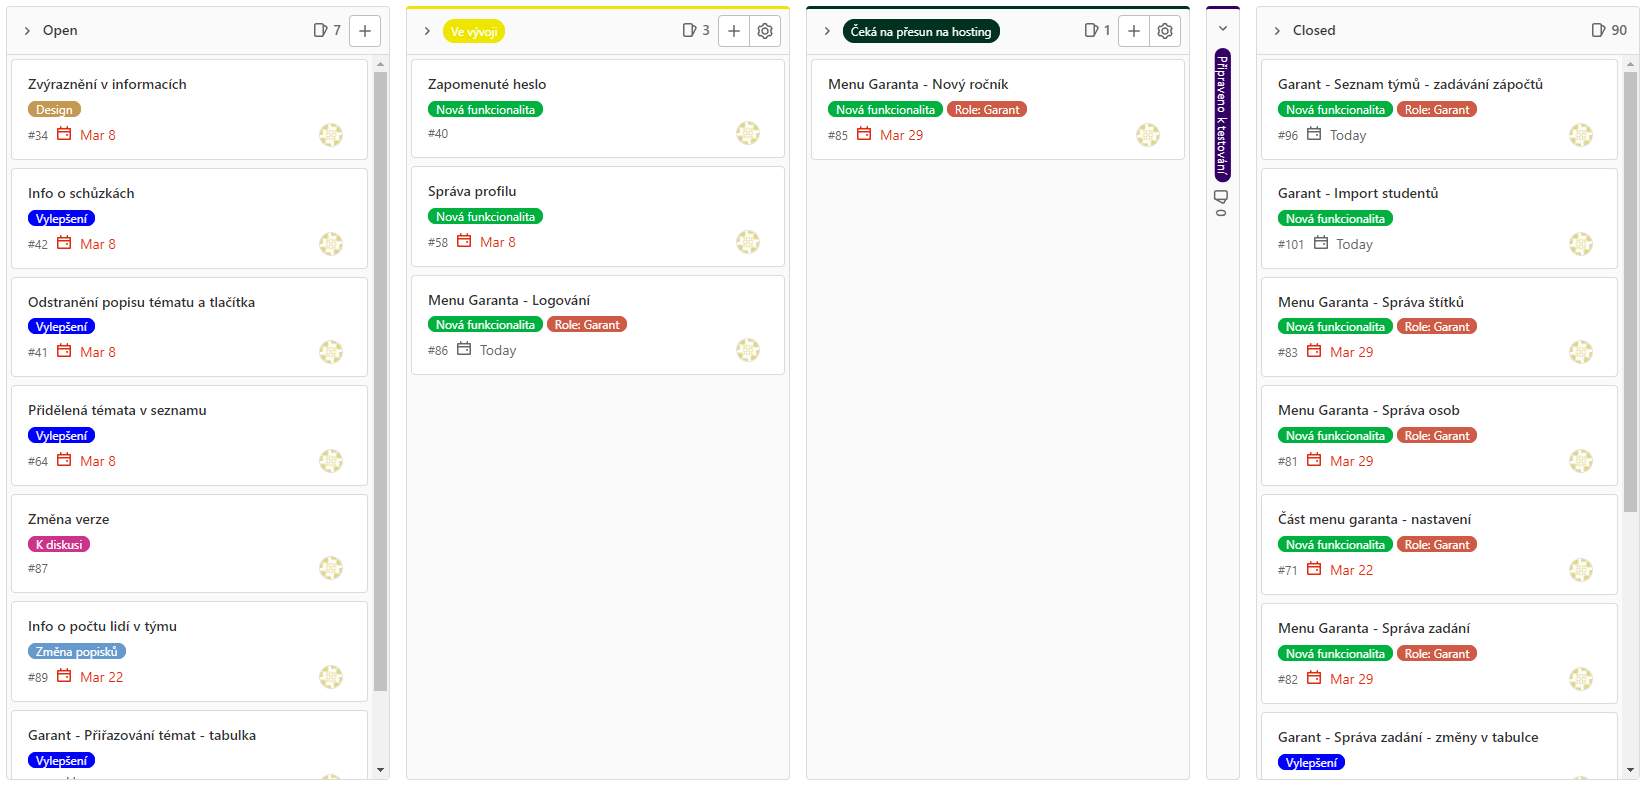
\includegraphics[width=\textwidth]{img/rizeni_projektu/kanban}
		\caption{Ukázka použití tabule s issues}
	\end{figure}
	\par V informačních technologiích se kanban používá ve velké míře pro organizaci různých úkolů a požadavků. Různé části vývoje si mezi sebou požadavek vyměňují a tím mění jeho stav.
	\par Například když vývojář dokončí práci na nové funkcionalitě, tak přesune příslušný rámeček ze sloupce \uv{Ve vývoji} do sloupce \uv{Připraveno k testování}. Tím se tester dozví, že je daný úkol připraven k testování a může si úkol přiřadit a pracovat na něm.
	\par V GitLabu je systém kanbanu implementován v souvislosti s issues a jejich štítky. Každý issue je zobrazen jeden rámeček na tabuli kanban, kam se automaticky po vytvoření issue promítne a po přidělení štítků zařadí do připravených sloupců.
	\par Propojenost s issue nám ulehčí práci s přepisováním jednotlivých požadavků do jiných nástrojů, které mají obdobné funkce.
\subsection{MantisBT}
	\par Mantis Bug Tracker je webová aplikace pro nahlašování a evidenci chyb (defektů) vytvořených v průběhu vývoje aplikace. Přidávané defekty lze velmi podrobně popsat, určit prioritu a štítkovat.
	\par MantisBT využíváme pro nahlašování objevených selhání nalezených především, ale ne výhradně pomocí komplexního automatizovaného testování aplikace. Na základě reportování defektů jsou následně žádány jejich opravy chyb a po opravě jsou znovu testovány. Pro naše potřeby používáme vlastní instalaci MantisBT, která je přístupná pro anonymně přihlášené, aby mohli v budoucnu nahlašovat defekty i uživatelé aplikace.
\chapter{Návrh aplikace}
	\section{Případy užití}
		\par Z podrobné specifikace požadavků vycházejí následující případy užití.
		\subsection{Nepřihlášený uživatel}
			\subsubsection{Přihlášení (UC.01)}
				\par Velká část aplikace jsou přístupné pouze uživatelům dle jejich role. To vytváří potřebu autentizace v naší aplikaci. Uživatel má možnost se přihlásit pomocí přihlašovací stránky pomocí registrované kombinace loginu a hesla. Pokud je uživatel autentizován, je přesměrován na domovskou obrazovku pro jeho konkrétní roli.
			\subsubsection{Zobrazení témat (UC.02-03)}
				\par Nepřihlášený uživatel (např. běžný student) si může zobrazit seznam volných témat v přehledu, kde se dozví základní informace o tématech.
				\par Tyto témata lze rozkliknout do podrobnější podoby, kde je zobrazen název, stručný popis, časová náročnost, doporučená velikost týmu, zadavatel a mentor zadání. Také lze stáhnout PDF soubor s podrobným zadáním.
			\subsubsection{Neúplné týmy (UC.04)}
				\par Nepřihlášený uživatel má k dispozici seznam neúplných týmů, které hledají nové členy. Případný student má k dispozici seznam obsazených rolí a kontakt na vedoucího týmu.
		\subsection{Přihlášený uživatel}
			\subsubsection{Odhlášení (UC.05)}
				\par Přihlášený uživatel má možnost ukončit svou relaci a odhlásit se. Po této akci je uživatel přesměrován na hlavní stránku nepřihlášeného uživatele.
		\subsection{Vedoucí týmu}
			\subsubsection{Schůzky týmu UC.06-09}
				\par 
		\subsection{Mentor}
		\subsection{Garant}
		\begin{figure}[h]
			\centering
			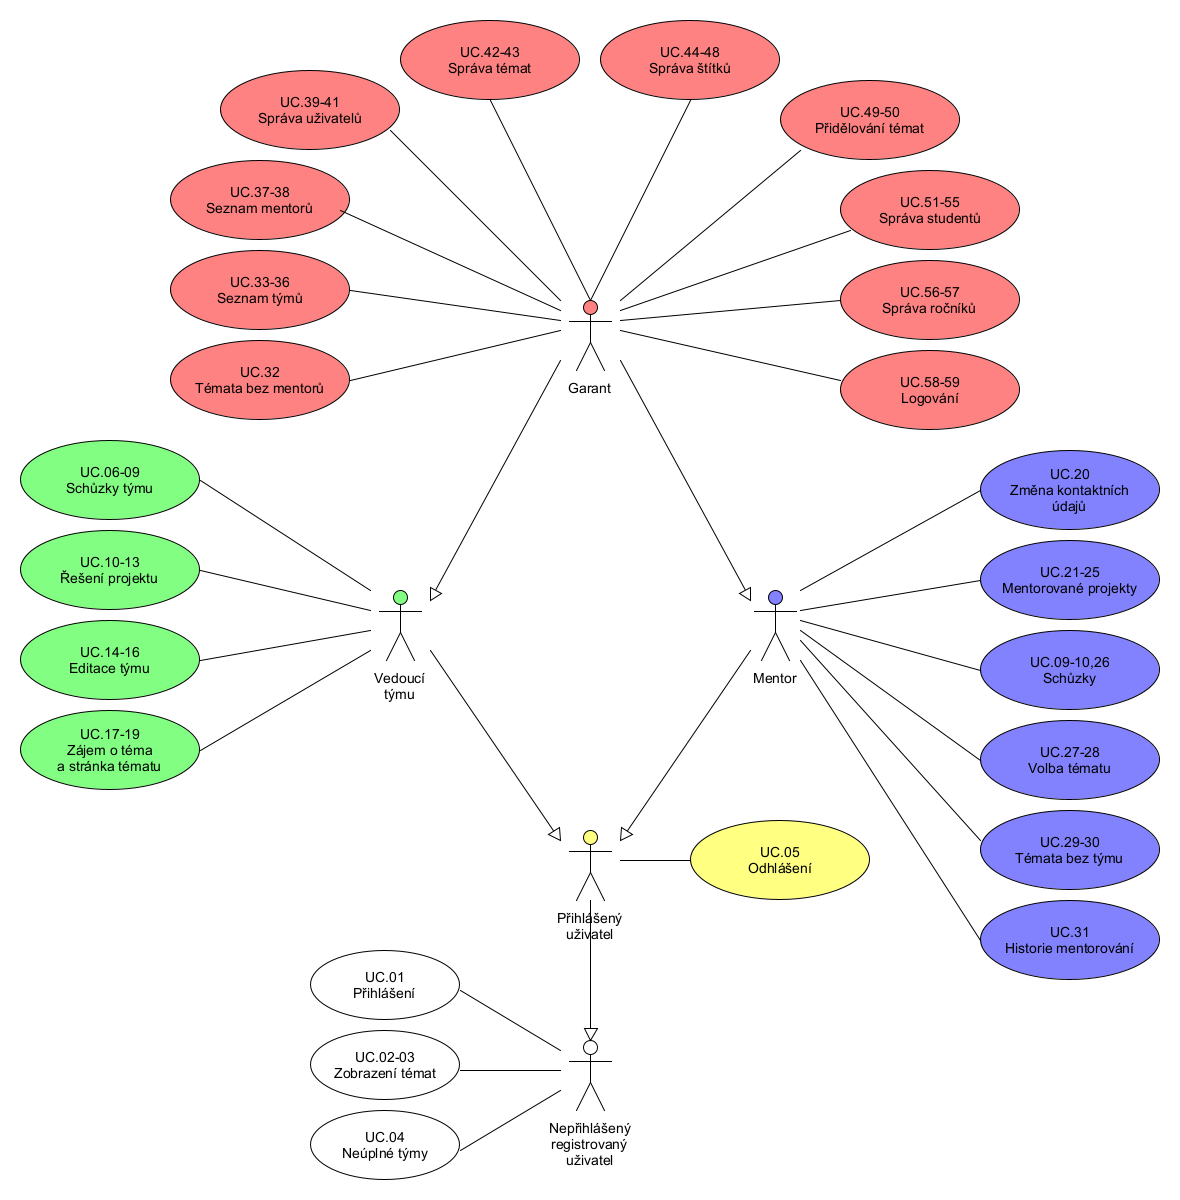
\includegraphics[width=0.8\textwidth]{img/use_case/use_case_diagram}
			\caption{Schéma případů užití}
		\end{figure}
	\section{Architektura aplikace}
		\subsection{MVP architektura}
		\par Architektura MVP (Model-View-Presenter) je třívrstvový návrh struktury aplikace pro rozdělení souborů dle funkčnosti s ohledem na rozšiřitelnost. MVP architektura se skládá z datové části (model), která se stará o práci s daty a umožňují vytvářet abstrakci nad jednotlivými strukturami. Například jednotlivé akce s databází v kontextu dat se kterými aplikace pracuje. Další část je aplikační vrstva (presenter), která řídí chod aplikace, předává data z šablon do modelů a naopak. Poslední vrstvou je vrstva prezentační. Ta se skládá z jednotlivých šablon a prezentace dat. Představuje tak rozhraní, přes které uživatel komunikuje s aplikací.
		\par Mezi další velice rozšířenou architekturou patří MVC architektura. Hlavním rozdílem mezi MVP a MVC architekturami je, zpracovávání vstupů od uživatele. V MVP architektuře jsou vstupy obsluhovány prezentovací vrstvou.
		\subsection{Komponenty aplikace v Nette}
		\par Komponenty jsou části aplikace, které vkládáme do stránek. Nejčastěji se jedná o formuláře, tabulky a další objekty, které je možné používat opakovaně.
		\par Nette má v sobě vestavěný komponentový systém, který umožňuje komponenty vkládat na stránky a někdy dokonce do jiných komponent, kdy se tak tvoří tzv. komponentový strom. Velkou výhodou je, že se komponenta tvoří až tehdy, kdy je opravdu použita. To těží výhodu zejména zpracování AJAX požadavků, kde je typicky výsledkem operace pouze část stránky, kdy není komponenta využita. Díky tomu se vůbec nevytváří tím šetří výkon serveru.
		\par Komponenty se vytváření v továrních funkcích v presenteru. Tyto funkce mají prototyp \texttt{createComponent<Name>(): Control} \cite{NetteComponents}.
		
		\subsubsection{Ukázka tovární metody v presenteru}
		\begin{lstlisting}[caption={Ukázka tovární metody v presenteru}]
class DefaultPresenter extends Nette\Application\UI\Presenter
{
	protected function createComponentPoll(): PollControl
	{
		$poll = new PollControl;
		$poll->items = $this->item;
		return $poll;
	}
}
		\end{lstlisting}
		 
		\par Komponentu lze definovat přímo v tovární metodě, ale pro účely znovupoužitelnosti je možné pro komponentu vytvořit vlastní třídu dědící třídu \texttt{Nette\textbackslash Application\textbackslash UI\textbackslash Control}.
	\section{Rozdělení aplikace dle způsobu užití}
		\subsection{Zadání}
			
		\subsection{Tým}
		\subsection{Projekt}
			
	\section{Databázová struktura}
		\par Struktura databáze musí obsahovat veškeré informace použitelné v softwarové podpoře a umožnit jejich snadné propojení. Dalších aspektem pro tvorbu struktury je použitý PHP framework, který využivá službu pro správu databázových dotazů a jejich optimalizaci. Pro jeho správnou funkci je potřeba mít strukturu databáze řádně připravenou včetně vytvořených indexů a propojení pomocí cizích klíčů.
		\par Databázová struktura musí respektovat, že požadavkem na aplikaci je prohlížení historie. To nás přivádí na strategii, že každá tabulka u které to bude potřeba bude provázána s tabulkou \texttt{PERIOD} jejíž řádky představují jednotlivé cykly TSP. Také se však vyskytuje problém u odstraňování řádek. Prakticky nebude možné z databáze cokoli odstraňovat, aby nebyla porušen konzistentní stav již proběhlých projektů. To je následně ve struktuře zapracováno v různých tabulkách sloupcem s příznakem, který určuje zda je prvek odstraněn nebo znepřístupněn.
		
		\begin{figure}[H]
			\centering
			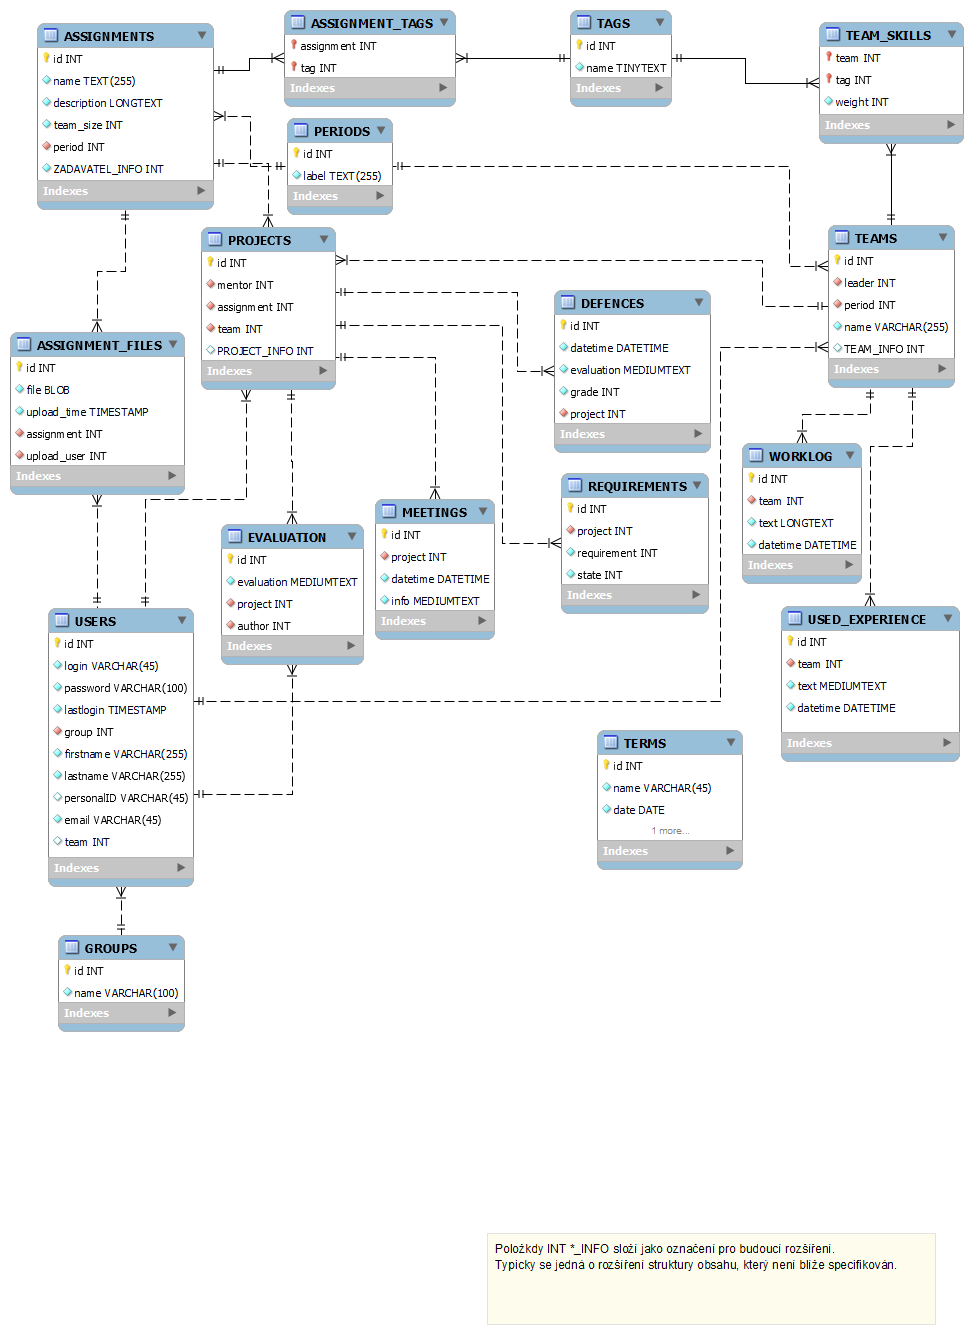
\includegraphics[width=0.8\textwidth]{img/database/database_model}
			\caption{Schéma databázové struktury}
		\end{figure}
		\subsection{Základní tabulky}
			\begin{itemize}
				\item USER -- Tabulka pro ukládání uživatelů, kteří mají/měli přístup do aplikace. Součástí této tabulky jsou přihlašovací údaje, role uživatele a následné propojení na další informace dle role uživatele.
				\item STUDENT -- Uživatelé s rolí \uv{Vedoucí} vycházejí ze záznamu tabulky \uv{STUDENT}, která obsahuje seznam všech studentů studujících předměty TSP.
				\item TEAM -- Tabulka pro evidenci týmů s jejich vedoucích.
				\item PROJECT -- Tabulka propojuje zadání z tabulky \uv{ASSIGNMENT} a týmu z tabulky \uv{TEAM}, tím vzniká projekt.
				\item CONTACT -- Tabulka pro evidenci informací a kontaktů na mentory a zadavatele.
				\item ASSIGNMENT -- Tabulka pro ukládání jednotlivých zadání.
				\item ASSIGNMENT\_INTEREST -- Tabulka pro evidenci zájmů o témata.
			\end{itemize}
		\subsection{Číselníkové tabulky}
		\par Tabulky sloužící jako číselník.
		\begin{itemize}
			\item TEAM\_ROLE -- Tabulka dostupných rolí v týmu.
			\item TAG -- Tabulka profilů pro použití v týmu a zadání.
			\item PROGRESS -- Tabulka se seznamem bodů, které tým v projektu plní.
			\item REQUIREMENT -- Tabulka se seznamem kritérií, která musí tým splnit.
			\item EXPERIENCE -- Tabulka využitých zkušeností
			\item PERIOD -- Tabulka jednotlivých cyklů aplikace a předmětů TSP.
		\end{itemize}
		\subsection{Spojovací tabulky}
			\begin{itemize}
				\item
				\item TEAM\_ROLE\_STUDENT -- Propojení mezi tabulkami \uv{TEAM\_ROLE} a \uv{STUDENT} pro realizaci N:M relace. 
				\item TEAM\_SKILL -- Propojení mezi tabulkami \uv{TAG} a \uv{TEAM} pro realizaci N:M relace. Tabulka specifikuje jaký tým má zvolenou jaký profil týmu.
				\item ASSIGNMENT\_TAG -- Propojení mezi tabulkami \uv{TAG} a \uv{ASSIGNMENT} pro realizaci N:M relace. Tabulka specifikuje jaké schopnosti bude tým potřebovat pro řešení tématu.
				\item PROGRESS\_STATE -- Propojení mezi tabulkami \uv{PROGRESS} a \uv{PROJECT} pro realizaci N:M relace. Tabulka eviduje postup v řešení projektu.
				\item REQUIREMENT\_STATE -- Propojení mezi tabulkami \uv{REQUIREMENT} a \uv{PROJECT} pro realizaci N:M relace. Tabulka eviduje plnění kritérií při řešení projektu.
				\item EXPERIENCE\_STATE -- Propojení mezi tabulkami \uv{EXPERIENCE} a \uv{PROJECt} pro realizaci N:M relace. Tabulka eviduje stav potvrzení využitých zkušeností.
			\end{itemize}
		\subsection{Další tabulky}
			\begin{itemize}
				\item ASSIGNMENT\_FILE -- Tabulka sloužící pro uložení PDF souborů s příslušnými informacemi.
			\end{itemize}
	\section{Uživatelské rozhraní}
\chapter{Realizace}
	\section{Adresářová struktura}
\chapter{Testování}

\chapter{Závěr}


%
% SEZNAM UKÁZEK KÓDU
%
\lstlistoflistings

% 
% PRO ANGLICKOU SAZBU JE NUTNÉ ZMĚNIT
% CITAČNÍ STYL!
%
\bibliographystyle{csplainnatkiv}
{\raggedright\small
\bibliography{literatura}
}

\end{document}
